\documentclass[12pt]{article}
\usepackage{amsmath}
\usepackage{graphicx}
\usepackage{wrapfig}
\usepackage{xcolor}
\usepackage{geometry}
\usepackage{hang}
\usepackage{newtxtext,newtxmath}
\usepackage{draftwatermark} % For watermark

% Watermark configuration (smaller font)
\SetWatermarkText{NCERT\\Not to be republished}
\SetWatermarkScale{0.4}          % Reduced font size
\SetWatermarkColor[gray]{0.9}    % Light gray background
\SetWatermarkAngle{45}           % Diagonal

\geometry{a4paper, margin=1in}

\title{}
\date{}

\begin{document}
\begin{figure}[h!]
    \begin{minipage}{0.45\textwidth}  % Set the width of the image
        \includegraphics[width=\textwidth]{sun.png}  % Replace 'image.png' with your image file name
    \end{minipage} \hfill
    \begin{minipage}{0.45\textwidth}  % Set the width of the text block
        \textbf{Name : K.KARTHIK} \\
    \textbf{Batch : cometfwc026} \\
  \textbf{Date :15 may 2025}
    \end{minipage}
\end{figure}
% Example 4
\noindent\textcolor{teal}{\large\textbf{Example 4:}} Find a relation between $x$ and $y$ such that the point $(x, y)$ is equidistant from the points $(7, 1)$ and $(3, 5)$.

\vspace{1em}
{\hangindent=2em
\noindent\textcolor{teal}{\textbf{Solution:}} Let $P(x, y)$ be equidistant from the points $A(7, 1)$ and $B(3, 5)$.\\
We are given that $AP = BP$. So, $AP^2 = BP^2$
\begin{align*}
(x - 7)^2 + (y - 1)^2 &= (x - 3)^2 + (y - 5)^2 \\
x^2 - 14x + 49 + y^2 - 2y + 1 &= x^2 - 6x + 9 + y^2 - 10y + 25 \\
x - y &= 2
\end{align*}
which is the required relation.
}

% Insert the image 'tree.png' on the right
\begin{wrapfigure}{r}{0.45\textwidth}
    \centering
    \vspace{-5pt}
    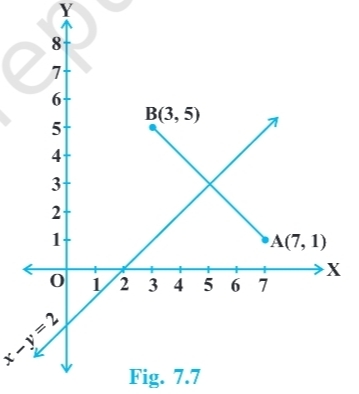
\includegraphics[width=0.43\textwidth]{tree.png}
    \vspace{-5pt}
\end{wrapfigure}

\vspace{1em}
\noindent\textcolor{teal}{\textbf{Remark:}} Note that the graph of the equation\\
$x - y = 2$ is a line. From your earlier studies,\\
you know that a point which is equidistant\\
from $A$ and $B$ lies on the perpendicular\\
bisector of $AB$. Therefore, the graph of\\
$x - y = 2$ is the perpendicular bisector of $AB$\\
(see Fig. 7.7).

\vspace{2em}

% Example 5
\noindent\textcolor{teal}{\large\textbf{Example 5:}} Find a point on the $y$-axis which \\
is equidistant from the points $A(6, 5)$ and \\
$B(-4, 3)$.

\vspace{1em}
{\hangindent=2em
\noindent\textcolor{teal}{\textbf{Solution:}} We know that a point on the $y$-axis is of the form $(0, y)$. So, let the point $P(0, y)$ be equidistant from $A$ and $B$. Then,
\begin{align*}
(6 - 0)^2 + (5 - y)^2 &= (-4 - 0)^2 + (3 - y)^2 \\
36 + 25 + y^2 - 10y &= 16 + 9 + y^2 - 6y \\
4y &= 36 \Rightarrow y = 9
\end{align*}
So, the required point is $(0, 9)$.
}

\end{document}
